\documentclass[aps,pra,reprint,superscriptaddress,amsmath,amssymb,longbibliography,floatfix]{revtex4-2}
\usepackage{amsthm}
\usepackage{bm,graphicx,booktabs}
\usepackage{xcolor}
\usepackage{hyperref}
\hypersetup{colorlinks=true,linkcolor=blue!45!black,citecolor=blue!45!black,urlcolor=blue!45!black,
  pdfauthor={Tingyu Zhang; Yan Cen}}
\newcommand{\ket}[1]{\lvert #1\rangle}
\newcommand{\bra}[1]{\langle #1\rvert}
\newcommand{\braket}[2]{\langle #1\mid #2\rangle}
\newcommand{\Tr}{\operatorname{Tr}}
\usepackage[UTF8,fontset=fandol]{ctex}
\newtheorem{theorem}{定理}
\newtheorem{lemma}{引理}
\newtheorem{proposition}{命题}
\renewcommand{\proofname}{证明}
\renewcommand{\acknowledgmentsname}{致谢}
\begin{document}

\title{多比特优雅联合测量的统一构造}
\hypersetup{pdftitle={多比特优雅联合测量的统一构造}}
\author{Tingyu Zhang}
\email{23300190021@m.fudan.edu.cn}
\affiliation{Department of Physics, Fudan University, Shanghai, China}
\author{Yan Cen}
\email[Corresponding author: ]{cenyan@fudan.edu.cn}
\affiliation{Department of Physics, Fudan University, Shanghai, China}
\date{October 31, 2026}
\begin{abstract}
连续调节优雅联合测量的共同 Bloch 半径，需要使其局部正四面体几何始终与完整正交归一测量基兼容。本文给出适用于全部整数 $n\ge5$ 的优雅联合测量显式连续族，以同一相位构造统一奇数与偶数情形。该族经过指定基准测量，保持测量基的正交归一性与固定局部正四面体方向，使共同 Bloch 半径连续覆盖 $[0,2r_E(n)]$，其中 $r_E(n)=\sqrt3/2^{n-1}$ 为基准半径。在固定相位表示中，本文完整分类由两值实相位生成元产生、经过该基准测量并在其邻域内保持共同半径正四面体几何的相位直线所允许的半径规律。由此证明，对每个 $n\ge5$，上界 $2r_E(n)$ 均可达到且在该模型内最优，并确定 $n=5$ 为该模型允许半径增强的最小规模。对每个偶数 $n\ge8$，本文进一步构造一个二维测量族，其两个坐标截面分别逐列恢复新增强族与已知余弦族。低维结果进一步揭示相位路径形状的作用：在同一相位表示下，当 $n=4$ 时，即使允许任意实相位生成元，所有经过基准测量并在其邻域内保持上述几何条件的相位直线仍不能增强半径，而一条显式弯曲路径可达到 $(1+1/\sqrt2)r_E(4)$。

\end{abstract}
\maketitle
\section{引言}
\label{intro:section}

纠缠投影测量同时受到全局基态正交性和局部约化态几何的约束。优雅联合测量（elegant joint measurement，EJM）将这两种性质结合起来：局部 Bloch 向量位于正四面体的顶点，而对应的全局态构成正交归一基。$n=2$ 的 EJM 最初出现于量子网络研究~\cite{Gisin2017}，并属于一族连接它与 Bell 态测量的连续测量~\cite{Tavakoli2021}。改变四面体半径会改变单比特约化谱，进而改变每个单比特与其余系统划分下的纠缠。将这种调节推广到更多比特，需要所有测量结果的局部几何始终与全局正交性兼容。

Pauli 轨道构造为这一问题提供了适合的框架~\cite{PauwelsPauli2026,PauwelsEJM2026}。在相应的相位正规形中，每个对角酉算符都会生成完整正交归一基，剩余约束集中于局部 Bloch 向量。Pauwels 与 Gisin 对每个 $n\ge2$ 给出了显式基准 EJM，其共同半径为
\begin{equation}
 r_E(n)=\frac{\sqrt3}{2^{n-1}},
 \label{intro:reference-radius}
\end{equation}
并构造了在 $|t|\le\pi/2$ 上满足 $r_E(n)\cos t$ 的偶数比特相位族~\cite{PauwelsGisin2026}。该文已将局部信号的来源解释为涉及单个计算基相位修正的干涉。其奇数比特分析将 $n\ge5$ 时经过指定基准点的显式可调族留作开放问题，并通过数值 Jacobian 秩识别出$n=3$ 时的局部孤立基准点。其它对称多比特构造允许更宽的局部几何~\cite{Ding2025,He2026}；本文保持每个比特上的一个固定正四面体，并要求所有比特和结果具有共同半径。

本工作的上一版对每个奇数 $n\ge5$ 给出了半径为 $r_E(n)(1-\sin t)$ 的显式增强族~\cite{Zhang2026Odd}。本文的构造不再区分奇偶：一个依赖四个二进制特征的新 Boolean 核，使同一半径规律适用于全部整数 $n\ge5$。它在 $t=0$ 逐列恢复基准测量，并连续连接局部极化为零与基准半径两倍这两个端点。这一增强自然引出其极限问题。为此，我们考察所有经过基准测量的两值实相位生成元，分类它们所允许的半径规律，证明两倍基准半径在该模型内最优；这一模型也包括四特征构造之外的生成元。

统一构造还使新增强变形与已知偶数比特余弦变形能够在同一相位表示中比较。我们考察两种调节能否在保持局部正四面体的同时独立进行。对每个偶数 $n\ge8$，一个显式的完整测量二维族给出了肯定答案，其两个坐标截面恰为这两种变形。$n=6$ 时，混合干涉阻碍了这一扩张；在相应的四颜色相位模型内，局部解只有两条相交分支。

更低维的情形进一步说明了直线相位路径何时不再足够。在 $n=2,3,4$ 时，两值相位直线均不能增强基准半径。$n=3$ 时，我们将 Pauwels 与 Gisin 的数值证据加强为精确的局部刚性证书。$n=4$ 时，即使允许任意实生成元，所有允许的直线仍不能增强半径，但一条显式弯曲路径可将半径增加至 $(1+1/\sqrt2)r_E(4)$。因此，在同一相位表示中改变路径形状即可突破$n=4$ 时的直线障碍。

第~II~节建立将这些问题归约为局部干涉条件的相位框架。第~III、IV~节给出统一构造及 Boolean 模型内的精确界。第~V~节建立它与已知偶数比特族的关系，第~VI~节解释低维障碍并给出$n=4$ 时的弯曲构造。各附录给出完整证明。

\section{相位框架与局部几何}
\label{core:framework}

为了在保持测量正交性的同时调节局部几何，将可调参数放入对角相位。对$n\ge2$，采用计算基$\ket{z_1\cdots z_n}$，其中$z_j\in\mathbb F_2$，门序沿用文献~\cite{PauwelsGisin2026}，矩阵乘积从右向左作用。记
\begin{align}
 C_n&=S(n)H_n,\qquad M[D]=C_nDH^{\otimes n},\nonumber\\
 S(n)&=\mathrm{CNOT}_{2\to1}\cdots\mathrm{CNOT}_{n\to n-1},
 \label{core:phase-family}
\end{align}
其中$H_n$只作用于末位比特，$D$为各对角元模长均为一的对角矩阵。由酉性，对每个这样的$D$，全部列$\ket{\psi_k}=M[D]\ket{k}$都构成正交完备测量。各列的局部几何由种子态$\ket{\psi_0}$决定：将列标签写为$k=(e_1,\ldots,e_{n-1},\sigma)$，其中$e\in\mathbb F_2^{n-1}$、$\sigma\in\mathbb F_2$，则有精确的Pauli轨道恒等式
\begin{equation}
 \ket{\psi_{e,\sigma}}=
 \left[\prod_{h=1}^{n-1}(Z_hZ_{h+1})^{e_h}\right]
 (X^{\otimes n})^\sigma\ket{\psi_0}.
 \label{core:orbit}
\end{equation}
这一轨道将种子的局部Bloch向量传递到全部测量列。要得到共同半径的正四面体，只需使种子的带符号局部分量相等。全文固定局部坐标：仅对末位比特的$Y$分量作符号调整，$\widetilde Y_n=-Y_n$；其余$\widetilde P$均等于相应的物理Pauli算符。因此，共同带符号分量$m\ge0$对应的种子Bloch向量为：$j<n$时$m(1,1,1)$，$j=n$时$m(1,-1,1)$。

相位变形从指定基点出发，其相位为
\begin{equation}
 \begin{aligned}
 f_0(z)&=\sum_{\ell=2}^n(-1)^\ell e_\ell(z)\\
 &=\begin{cases}0,&z=0,\\ |z|-1,&z\ne0,\end{cases}\pmod4.
 \end{aligned}
 \label{core:reference-phase}
\end{equation}
其中$e_\ell$为基本对称多项式，$|z|$为Hamming重量。基点测量取$D_0(z)=i^{f_0(z)}$，其半径为
\begin{equation}
 c_n=2^{1-n},\qquad r_E(n)=\sqrt3\,c_n.
 \label{core:reference-radius}
\end{equation}

为计算种子的带符号分量，将种子态分解为背景态与物理全零串处的单点修正。对$\mathbb F_2^n$上任意实函数$\Theta$，定义
\begin{align}
 \ket{\chi_\Theta}&=2^{-n/2}\sum_z i^{|z|}e^{i\Theta(z)}\ket z,\nonumber\\
 D_\Theta(z)&=\begin{cases}1,&z=0,\\
 i^{f_0(z)}e^{i\Theta(z)},&z\ne0.
 \end{cases}
 \label{core:background}
\end{align}
种子态严格满足
\begin{equation}
 \ket{\psi_0}=-iC_n\left[\ket{\chi_\Theta}
 +2^{-n/2}\big(i-e^{i\Theta(0)}\big)\ket{0^n}\right].
 \label{core:defect-state}
\end{equation}
无论如何表示$\Theta$，该修正只改变一个物理输入的振幅。

\begin{lemma}[局部相位机制]
\label{core:mechanism}
对带符号的局部Pauli算符，记
\begin{equation}
 R=C_n^\dagger\widetilde P C_n=i^kX^aZ^b,\quad
 h=a\oplus b,\quad\Gamma=i^{k-|a|},
 \label{core:pauli-notation}
\end{equation}
并令$B_R=\bra{\chi_\Theta}R\ket{\chi_\Theta}$，则
\begin{equation}
 \langle\widetilde P\rangle
 =B_R+c_n\operatorname{Re}\!\left[
 \Gamma e^{-i\Theta(a)}\big(i-e^{i\Theta(0)}\big)\right].
 \label{core:signal}
\end{equation}
若所有带符号期望均等于$m\ge0$，则每个测量列的真实单比特约化态为
\begin{equation}
 \rho_{j,e,\sigma}
 =\frac12\left[I+\sqrt3m\,\mathbf v_{j,\kappa_j,\sigma}
 \cdot\boldsymbol\sigma\right],
 \label{core:bloch-orbit}
\end{equation}
其中$e_0=e_n=0$、$\kappa_j=e_{j-1}\oplus e_j$，且
\begin{equation}
 \begin{aligned}
 \mathbf v_{j,q,s}&=\frac1{\sqrt3}
 \big((-1)^q,\epsilon_j(-1)^{q+s},(-1)^s\big),\\
 \epsilon_j&=\begin{cases}1,&j<n,\\-1,&j=n.\end{cases}
 \end{aligned}
 \label{core:vertices}
\end{equation}
对每个$j$，这四个单位向量构成正四面体，每个标签$(q,s)$恰出现$2^{n-2}$次。
\end{lemma}

所有拉回算符均满足$a\ne0$，所以式\eqref{core:defect-state}中的修正对局部期望没有对角贡献；两个交叉项给出式\eqref{core:signal}。由式\eqref{core:orbit}中的轨道算符作共轭，即得式\eqref{core:vertices}的四面体符号。附录\ref{core:appendix}给出逐门拉回及约化态推导。

对Boolean相位$\Theta=tq$且$q(0)=1$，拉回算符分为两类：I类满足$\Gamma=-i$、$h\cdot a=1$；II类满足$\Gamma=-1$、$h\cdot a=0$。定义归一化Walsh系数
\begin{equation}
 \begin{aligned}
 W_q(h)&=2^{-n}\sum_z(-1)^{q(z)\oplus h\cdot z},\\
 D_aq(z)&=q(z)\oplus q(z\oplus a).
 \end{aligned}
 \label{core:walsh-def}
\end{equation}
则背景项为
\begin{equation}
 B_R(t)=\begin{cases}
 -\sin t\,W_q(h),&\text{I类},\\
 -\sin^2(t/2)\,W_{D_aq}(h),&\text{II类}.
 \end{cases}
 \label{core:boolean-background}
\end{equation}
这些公式将背景项写成相位函数及其导数的Walsh系数。

\section{全部\texorpdfstring{$n\ge5$}{n >= 5}的统一族}
\label{core:unified}

式\eqref{core:signal}给出两项设计要求：消去所有背景项$B_R(t)$，并使剩余交叉项相等。对Boolean相位，前者化为式\eqref{core:boolean-background}中的Walsh消去条件，后者确定局部翻转处的取值$q(a)$。对每个整数$n\ge5$，四个线性特征将这两项要求归约为同一个四位核上的条件。定义两个内部奇偶块
\begin{equation}
 \begin{aligned}
 E_n&=\{2,4,\ldots\}\cap[2,n-2],\\
 O_n&=\{3,5,\ldots\}\cap[2,n-2],
 \end{aligned}
\end{equation}
以及四个线性特征
\begin{align}
 x&=z_1\oplus z_{n-1},& b&=\bigoplus_{j\in E_n}z_j,\nonumber\\
 c&=\bigoplus_{j\in O_n}z_j,& s&=z_1\oplus z_n.
 \label{core:features}
\end{align}
记$\mathcal L_nz=(x,b,c,s)$。两个内部块均非空，四个特征线性无关。在$\mathbb F_2^4$上取
\begin{equation}
 F(x,b,c,s)=\begin{cases}
 1\oplus(1\oplus c)(x\oplus b),&s=0,\\
 b\oplus xc,&s=1.
 \end{cases}
 \label{core:kernel}
\end{equation}
令
\begin{equation}
 q_n(z)=F(\mathcal L_nz),\qquad
 d_n(z)=q_n(z)-\delta_{z,0}.
 \label{core:support}
\end{equation}
这里的减法取整数意义。因为$F(0)=1$，$d_n$仍为Boolean函数。被移除的只有物理全零串，不是整个纤维$\mathcal L_nz=0$。

图~\ref{fig:unified}(a)展示同一四特征核如何确定每个$n\ge5$的相位；图(b)给出以$r_E(n)$归一化的半径变化。
\begin{figure*}[tbp]
  \centering
  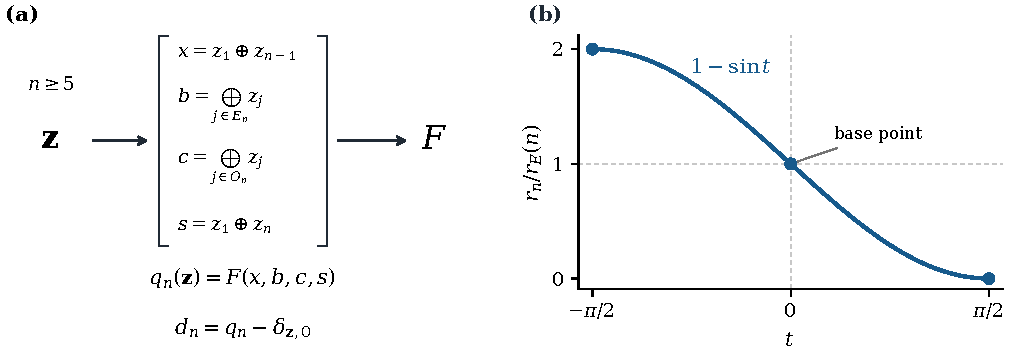
\includegraphics[width=\textwidth]{figures/fig1_unified.pdf}
  \caption{Unified phase deformation for every $n\geq5$.
  (a) Four linear Boolean features feed the same kernel $F$; the only removed support point is the physical string $\mathbf z=0$.
  The blocks $E_n$ and $O_n$ contain the even and odd indices in $[2,n-2]$, respectively.
  (b) The normalized common Bloch radius $r_n(t)/r_E(n)=1-\sin t$ on $[-\pi/2,\pi/2]$, where $r_E(n)=\sqrt3/2^{n-1}$ is the reference radius.
  From left to right, the marked points give the enhanced endpoint, the specified EJM at $t=0$, and the endpoint with maximally mixed one-qubit marginals.}
  \label{fig:unified}
\end{figure*}

\begin{theorem}[统一增强族]
\label{core:unified-theorem}
对每个整数$n\ge5$，令
\begin{equation}
 D_{n,t}(z)=i^{f_0(z)}e^{itd_n(z)},\qquad
 M_n(t)=C_nD_{n,t}H^{\otimes n}.
 \label{core:unified-measurement}
\end{equation}
对每个实数$t$，全部列均构成正交归一基，其单比特约化态由式\eqref{core:bloch-orbit}给出，其中
\begin{equation}
 m_n(t)=c_n(1-\sin t),\qquad
 r_n(t)=r_E(n)(1-\sin t).
 \label{core:radius}
\end{equation}
四面体方向与$t$无关。在区间
\begin{equation}
 J=[-\pi/2,\pi/2],\qquad r_n(J)=[0,2r_E(n)],
 \label{core:interval}
\end{equation}
半径连续且严格递减。$t=0$逐列恢复基点测量；$t=-\pi/2$达到半径$2r_E(n)$；$t=\pi/2$时全部单比特约化态均为$I/2$。
\end{theorem}

\begin{proof}
证明将随维数变化的特征映射与六个固定的四位消去恒等式分开。首先，形如
\begin{equation}
 2^{-n}\sum_z(-1)^{h\cdot z}G(\mathcal L_nz)
 \label{core:pairing-sum}
\end{equation}
的和式，在$h$不属于$\mathcal L_n$行空间时为零：取$\mathcal L_nw=0$、$h\cdot w=1$的平移$z\mapsto z\oplus w$，每一项的符号均反转。当$h$属于行空间时，写成$h=\mathcal L_n^TH$，利用各纤维等大，将式\eqref{core:pairing-sum}化为$2^{-4}\sum_v(-1)^{H\cdot v}G(v)$。对$q_n$的导数同样适用，因为$D_aq_n=(D_AF)\circ\mathcal L_n$，其中$A=\mathcal L_na$。

其次，逐门拉回表中的局部字符只留下以下条件：
\begin{align}
 W_F(9)&=W_F(11)=W_F(15)=0,\nonumber\\
 W_{D_6F}(6)&=W_{D_7F}(13)=W_{D_7F}(11)=0.
 \label{core:six-cancellations}
\end{align}
整数按$(x,b,c,s)$编码，$x$为最高位；Walsh系数的归一化因子为$2^{-4}$。六个和式均可通过特征位配对消去。附录~\ref{core:alln-classification}给出有限计算，并证明这六式覆盖每个$n\ge5$的全部局部分量，包括$n=5,6,7$的额外残留项。由式\eqref{core:boolean-background}，$B_R(t)$恒为零。

最后，所有I类翻转均满足$F(\mathcal L_na)=0$，所有II类翻转均满足$F(\mathcal L_na)=1$。式\eqref{core:signal}分别化为
\begin{align}
 c_n\operatorname{Re}[-i(i-e^{it})]&=c_n(1-\sin t),\nonumber\\
 c_n\operatorname{Re}[-e^{-it}(i-e^{it})]&=c_n(1-\sin t).
\end{align}
引理\ref{core:mechanism}把种子恒等式传递到全部测量列。端点、基点与精确像的结论由对角相位以及$\sin t$在$J$上的严格单调性得到。
\end{proof}

该增强具有直接的单比特纠缠含义。所有测量结果、所有$1|(n-1)$划分共享同一局部谱
\begin{equation}
 \lambda_\pm=\frac{1\pm r_n(t)}2,
 \qquad \operatorname{Tr}\rho_j^2=\frac{1+r_n(t)^2}{2}.
 \label{core:spectrum}
\end{equation}
相应的熵为$h_2((1+r_n(t))/2)$，其中$h_2(p)=-p\log_2p-(1-p)\log_2(1-p)$，端点值按连续性定义。Bloch半径增加时，这一二分纠缠下降。$t=\pi/2$时，式\eqref{core:defect-state}的单点修正消失；$t=-\pi/2$时，其干涉产生基点两倍的局部信号。四个线性特征足以表示全部$n$的相位，但提取这些特征仍依赖物理寄存器的大小。




\section{Boolean 相位直线的精确界}
\label{bound:section}

上述增强族还达到了一个更大相位变形类别中的最大半径。本节允许物理输入串上的任意 Boolean 函数，不要求特定压缩结构，也不预设背景态的条件。令
\begin{equation}
 \begin{gathered}
 M_d(t)=C_n\operatorname{diag}_{z}
 \bigl(i^{f_0(z)}e^{itd(z)}\bigr)H^{\otimes n},\\
 d:\mathbb F_2^n\longrightarrow\{0,1\},\qquad d(0)=0.
 \end{gathered}
 \label{bound:line}
\end{equation}
若在包含 $t=0$ 的某个开区间内，各局部 Pauli 轨道形成共同半径的正四面体，就称这条直线为可容许直线。这一条件针对完整测量；酉分解已保证每个实参数处的正交归一性。

\begin{theorem}[四律与 Boolean 直线的精确界]
\label{bound:theorem}
设 $n\ge3$，$d$ 为可容许直线的生成元，并记 $c_n=2^{1-n}$。全部带符号局部分量在所有实数 $t$ 上具有同一值 $m_d(t)$，且存在一个固定的 $(s,k)\in\{0,1\}^2$，使
\begin{equation}
 m_d(t)=c_n\bigl[(1-s)+s\cos t-k\sin t\bigr].
 \label{bound:four-laws}
\end{equation}
因此，$m_d/c_n$ 只有四种可能的函数形式：$1$、$\cos t$、$1-\sin t$ 和 $\cos t-\sin t$；每个维数中未必都能实现全部四种形式。另外，对每个 $n\ge2$，记 $r_E(n)=\sqrt3\,c_n$，则可容许直线中的精确最大半径为
\begin{equation}
 \max_{\substack{d\ \text{admissible}\\t\in\mathbb R}}r_d(t)
 =\begin{cases}
 r_E(n),&n=2,3,4,\\
 2r_E(n),&n\ge5.
 \end{cases}
 \label{bound:sharp-max}
\end{equation}
两种最大值均能达到。
\end{theorem}

在基点处，这些分量全部等于正数 $c_n$，故规则性要求它们在基点邻域相等。每个分量均为 $1$、$\cos t$ 和 $\sin t$ 的线性组合，邻域中的相等因而延伸到全部实数 $t$。特别地，
\begin{equation}
 r_d(t)=\sqrt3\,|m_d(t)|.
 \label{bound:radius}
\end{equation}
在 $m_d\ge0$ 的区间内，四面体保持原有取向。

关键约束来自两类拉回 Pauli 算符的系数比较。令 $q=d+\delta_0$，则 $q$ 仍为 Boolean 函数且 $q(0)=1$，沿用式~\eqref{core:walsh-def} 的 Walsh 系数与 Boolean 导数定义。
I 类分量的余弦系数为 $c_nq(a)$，II 类分量的正弦系数为 $-c_nq(a)$。对 $n\ge3$，两类均非空，因此分量相等迫使 I 类的所有翻转值为同一个 $s$，II 类的所有翻转值为同一个 $k$。其余系数相等恰好等价于
\begin{equation}
 \begin{aligned}
 q(a)&=s,& W_q(h)&=c_n(s+k-1)&&({\rm I}),\\
 q(a)&=k,& W_{D_aq}(h)&=2c_n(s+k-1)&&({\rm II}).
 \end{aligned}
 \label{bound:conditions}
\end{equation}
这些条件给出式~\eqref{bound:four-laws}，并且也是充分条件。对增强规律 $1-\sin t$，这些条件迫使两类 Walsh 系数均为零，从式~\eqref{core:boolean-background} 得到背景恒为零。

四个归一化函数的绝对值最大值依次为 $1$、$1$、$2$ 和 $\sqrt2$，由此得到全部 $n\ge3$ 的上界 $2r_E$。低维条件更强：$n=3$ 时，两条 I 类字符方程迫使 $s=k=0$；$n=4$ 时，四条此类方程相加得到 $4k=0$，只余常值与余弦规律。$n=2$ 时没有 II 类，单独计算后同样只允许这两种规律。附录~\ref{bound:appendix} 给出系数计算与这些解析排除。低维上界在基点达到，而统一增强族对每个 $n\ge5$ 都在 $t=-\pi/2$ 达到 $2r_E$。

因此，沿经过指定基点的 Boolean 相位直线增加半径，所需的最小系统规模为 $n=5$。这一结论也涵盖任意两值实对角生成元：减去其在 $z=0$ 的值可去除整体相位，再缩放或反向参数 $t$，便得到式~\eqref{bound:line}。一般多值相位直线和弯曲路径需要另行分析；后文 $n=4$ 的结果具体展示了这种区别。

\section{包含已知偶数比特族的母族}
\label{embed:section}

统一构造和已知偶数比特族给出了经过同一基准测量的两个相位方向。本节考察这两个方向能否在保持正四面体几何的同时独立变化。为在完整测量层面比较它们，先用第~\ref{core:framework}~节的记号表达该余弦族。对偶数 $n$，沿用
$E=\{2,4,\ldots,n-2\}$，定义
\begin{equation}
 q_A(z)=\prod_{j\in E}(1-z_j),\qquad d_A(z)=q_A(z)-\delta_{z,0}.
 \label{embed:and-support}
\end{equation}
对角相位 $i^{f_0(z)}e^{i\alpha d_A(z)}$ 恰为 Pauwels 与 Gisin 的偶数比特族~\cite{PauwelsGisin2026}，其参数对应为 $\alpha=\pi\tau/2$。背景仅依赖偶数内部坐标，而表~\ref{core:pullback-table} 中每个字符 $h$ 均含有 $E$ 之外的坐标；翻转该坐标便使背景期望成对消去。此外，I 类有 $q_A(a)=1$，II 类有 $q_A(a)=0$。因此，式~\eqref{core:signal} 给出共同带符号分量 $c_n\cos\alpha$，在 $|\alpha|\le\pi/2$ 上得到 $r=r_E(n)\cos\alpha$。这一论证包括 $n=2$ 时的空乘积 $q_A=1$，以及 $n=4$ 时的 $q_A=1-z_2$。

对偶数 $n\ge8$，该余弦族与统一增强族是同一二维族的坐标截面。令 $d_B=d_n$ 为式~\eqref{core:support} 中的支持，定义
\begin{align}
 D_{\alpha,\beta}(z)&=i^{f_0(z)}e^{i\alpha d_A(z)+i\beta d_B(z)},\notag\\
 M_n(\alpha,\beta)&=C_nD_{\alpha,\beta}H^{\otimes n}.
 \label{embed:measurement}
\end{align}
图~\ref{fig:embedding} 展示这一构造。
\begin{figure*}[tbp]
  \centering
  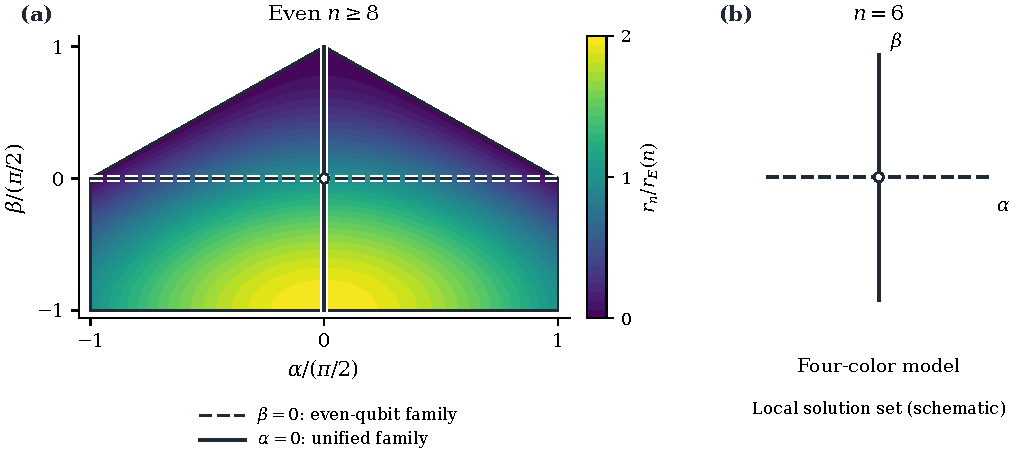
\includegraphics[width=\textwidth]{figures/fig2_embedding.pdf}
  \caption{偶数比特母族的两个精确截面。
  (a) 偶数 $n\geq8$ 的参数域 $\Omega$，颜色表示 $r_n/r_E(n)=\cos\alpha-\sin\beta$。
  虚线截面 $\beta=0$ 逐列恢复已知偶数族，实线截面 $\alpha=0$ 逐列恢复统一增强族。空心圆为共同基点。
  (b) $n=6$ 时四联合颜色加独立零点相位模型的局部解集示意：两支在基点交叉。 绘图代码由 OpenAI Codex（GPT-6）辅助编写，并按文中公式核对。}
  \label{fig:embedding}
\end{figure*}

\begin{theorem}[二维包含]
\label{embed:theorem}
对每个偶数 $n\ge8$，式~\eqref{embed:measurement} 在全部实参数 $\alpha,\beta$ 上定义正交完备测量，其全部种子带符号分量均为
\begin{equation}
 m_n(\alpha,\beta)=c_n(\cos\alpha-\sin\beta).
 \label{embed:component}
\end{equation}
在参数域
\begin{equation}
 \Omega=\left\{(\alpha,\beta): |\alpha|\le\frac\pi2,\quad
 -\frac\pi2\le\beta\le\frac\pi2-|\alpha|\right\}
 \label{embed:domain}
\end{equation}
上，该测量保持式~\eqref{core:bloch-orbit} 的固定局部正四面体，且
\begin{align}
 r_n(\alpha,\beta)&=r_E(n)(\cos\alpha-\sin\beta),\notag\\
 r_n(\Omega)&=[0,2r_E(n)].
 \label{embed:radius}
\end{align}
$\beta=0$ 截面逐列恢复已知偶数比特族，$\alpha=0$ 截面逐列恢复定理~\ref{core:unified-theorem} 的统一增强族。两个参数方向在有序测量投影层面独立。
\end{theorem}

证明的关键在于联合背景消去。令 $u=e^{i\alpha}$、$v=e^{i\beta}$，则施加 $-iC_n$ 之前的种子为
\begin{equation}
 2^{-n/2}\left[\sum_z i^{|z|}u^{q_A(z)}v^{q_B(z)}\ket z
 +(i-uv)\ket{0^n}\right],
 \label{embed:seed}
\end{equation}
其中 $q_B=q_n$。每个 I 类翻转满足 $(q_A(a),q_B(a))=(1,0)$，每个 II 类翻转满足 $(q_A(a),q_B(a))=(0,1)$。因此两类的缺陷贡献相同，因为
\begin{align}
 \operatorname{Re}[-iu^{-1}(i-uv)]
 &=\cos\alpha-\sin\beta,\notag\\
 \operatorname{Re}[-v^{-1}(i-uv)]
 &=\cos\alpha-\sin\beta.
 \label{embed:defect}
\end{align}
I 类翻转不改变 $q_A$，其背景退化为已证明消失的 $q_B$ 背景。对 II 类，将背景和按 AND 差分 $q_A(z)-q_A(z\oplus a)=1,0,-1$ 分为三个扇区。第一扇区的全部偶数内部位为零。当 $n\ge8$ 时，奇数内部块至少含两位；该块上的非常值字符可通过保持奇偶性的双位翻转消去。最后仅剩六个固定四位和，其系数均精确为零。附录~\ref{embed:appendix} 给出完整分类和六个有限恒等式。由此对任意 $n$ 证明式~\eqref{embed:component}，再由轨道公式得到全部约化态。

在 $\Omega$ 上，$\sin\beta\le\cos\alpha$，且 $\cos\alpha-\sin\beta\le2$；$\alpha=0$ 截面已取尽零至二的全部值。两轴的完整测量恒等式直接来自式~\eqref{embed:measurement} 的对角元。为确认参数在取投影后仍然独立，考虑对角输入相位的无穷小变化 $A$：它仅产生列相位，当且仅当存在对角 $B$ 使 $AH^{\otimes n}=H^{\otimes n}B$。Hadamard 矩阵的所有元素均非零，故 $A,B$ 必为同一标量。$(d_A,d_B)$ 在 $0,e_1,e_1\oplus e_2$ 依次取 $(0,0),(1,0),(0,1)$，因此两个方向的非零线性组合不可能为标量。

\begin{proposition}[$n=6$ 时的分支交叉]
\label{embed:six-proposition}
当 $n=6$ 时，式~\eqref{embed:measurement} 的直接叠加具有相同带符号分量，当且仅当 $\sin\alpha\sin\beta=0$。更一般地，允许对 $(q_A,q_B)$ 的四种取值分别赋相位，并独立改变物理零串的相位；在指定 EJM 附近，该模型中的规则测量恰为两条原有单参数分支。
\end{proposition}
此时奇数内部块只有一位。$X_3$ 与 $X_4$ 的归一化背景期望额外出现 $-\sin\alpha\sin\beta/8$，其余分量仍取共同缺陷值。附录~\ref{embed:appendix} 求解了完整的局部颜色方程。因此，$n=6$ 时已有增强族，但这里的二维扩张在局部只保留两条坐标轴的交叉。

\section{低维刚性与弯曲变形}
\label{low:section}
\begin{figure}[htbp]
  \centering
  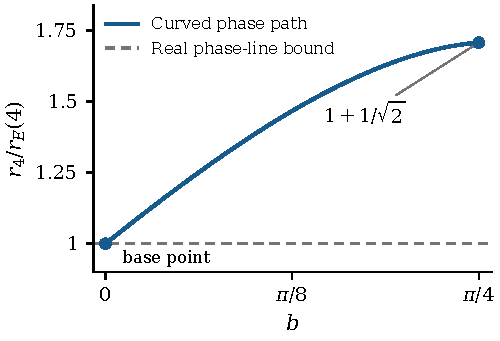
\includegraphics[width=\columnwidth]{figures/fig3_curved.pdf}
  \caption{$n=4$ 时沿显式弯曲相位路径的增强。
  实线由闭式根在 $0\leq b\leq\pi/4$ 上直接计算得到，满足
  $r_4/r_E(4)=\cos[b+\delta(b)]-\sin\delta(b)$，从 $1$ 严格增至 $1+1/\sqrt2$。
  水平虚线表示所有经过指定基点的实相位直线的半径上界。 绘图代码由 OpenAI Codex（GPT-6）辅助编写，并按文中公式核对。}
  \label{fig:curved}
\end{figure}


在固定相位表示中，$n=5$ 这一阈值有一个几何解释。$n=3$ 的指定测量在局部孤立。
$n=4$ 时的规则性方程允许变形，但每一条可行相位直线均不能增加半径；经过同一点的弯曲路径则可以实现增强。

\begin{proposition}[$n=3$ 时的局部刚性]
\label{low:rigidity}
在固定 Pauli 轨道表示中，去除整体相位后，$n=3$ 的指定 EJM 在其相位向量的一个邻域内是孤立的。
\end{proposition}
七个独立相位对应八个带符号局部分量差，其中七个约束的导数在指定点的行列式为
$1/4096$。由逆函数定理，这七个方程的零点局部孤立。
指定点的全部带符号分量均为 $1/4$，故在其邻域内，平方规则性条件与带符号分量相等条件等价。
附录~\ref{low:app-rigidity} 的精确 Jacobian 将文献~\cite{PauwelsGisin2026}
报告的数值秩转化为解析的局部结论。

对于 $n=4$，将任意相位直线写为
\begin{equation}
 M_d(t)=C_4\operatorname{diag}
 \bigl(i^{f_0(z)}e^{itd_z}\bigr)H^{\otimes4},\qquad d_0=0.
 \label{low:line}
\end{equation}
规范 $d_0=0$ 仅去除公共相位，其余 15 个分量可以取任意实数。

图~\ref{fig:curved} 比较相位直线的半径上界与下述弯曲增强。
\begin{theorem}[$n=4$ 时的直线与弯曲增强]
\label{low:theorem}
若直线~\eqref{low:line} 在 $t=0$ 的一个邻域内始终给出共同半径的规则四面体测量，则存在实数 $\omega$ 使
\begin{equation}
 r_d(t)=r_E(4)|\cos(\omega t)|\le r_E(4).
 \label{low:line-bound}
\end{equation}
另一方面，经过同一测量的显式弯曲相位路径满足
\begin{equation}
 r_4\bigl([0,\pi/4]\bigr)
 =\left[r_E(4),\left(1+\frac1{\sqrt2}\right)r_E(4)\right],
 \label{low:curve-range}
\end{equation}
且半径沿该路径严格递增。
\end{theorem}

直线路径的障碍强于 Boolean 模型上界。完整线性化约束核为四维；
二阶条件排除其中一个方向，仅留下一个候选比例，非零三阶项进一步排除该候选。
剩余方向组成两个平面，两者均只产生式~\eqref{low:line-bound} 的余弦规律。
附录~\ref{low:app-lines} 给出明确分类。

为构造能够离开这两个平面的路径，允许两个独立实参数 $b,\delta$，
取式~\eqref{low:masks} 中的两个固定整数掩码 $u,v$，令 $\theta_z=bu_z+\delta v_z$。
在这些相位下，种子的带符号物理 Pauli 分量只有两种取值：十个分量等于 $T/8$，
而 $X_1$ 与 $-Y_4$ 的分量等于 $H/8$，其中
\begin{align}
 T&=\cos(b+\delta)-\sin\delta,\nonumber\\
 H&=\cos b+2\sin\delta\cos b+4\sin b\cos b.
 \label{low:two-components}
\end{align}
这些恒等式在选取路径之前就成立。因此，带符号规则性条件为 $H=T$，
它是关于 $\tan(\delta/2)$ 的二次方程。

经过 $(b,\delta)=(0,0)$ 的根分支具有如下闭式表达。对 $0\le b\le\pi/4$，定义
\begin{align}
 A(b)&=\cos b(1+2\sin b),\nonumber\\
 B(b)&=2\cos b+\sin b+1,\qquad
 C(b)=2\sin b\cos b,\nonumber\\
 \delta(b)&=-2\arctan\frac{2C(b)}
 {B(b)+\sqrt{B(b)^2-4A(b)C(b)}}.
 \label{low:delta}
\end{align}
由此得到相位路径及测量
\begin{equation}
 \begin{aligned}
 \theta_z(b)&=bu_z+\delta(b)v_z,\\
 M_4(b)&=C_4\operatorname{diag}
 \bigl(i^{f_0(z)}e^{i\theta_z(b)}\bigr)H^{\otimes4}.
 \end{aligned}
 \label{low:curve}
\end{equation}
因此，在整条显式路径上，全部带符号分量始终相等。
结合酉性与 Pauli 轨道关系，即得到完整测量及其固定局部四面体。其共同半径为
\begin{equation}
 r_4(b)=r_E(4)\bigl[\cos\bigl(b+\delta(b)\bigr)-\sin\delta(b)\bigr].
 \label{low:curve-radius}
\end{equation}
在闭区间 $0\le b\le\pi/4$ 上，式~\eqref{low:delta} 中根号内的量和分母均严格为正。
附录~\ref{low:app-curve} 证明该分支在此区间内有良好定义，且半径严格递增。
在 $b=0$ 时两个角度均为零，因而逐列恢复原测量。
另一端点满足 $\delta(\pi/4)=-\pi/4$，给出式~\eqref{low:curve-range} 的上端点。
弯曲路径离开可行直线方向组成的两个平面，并满足 $r'_4(0)=\sqrt3/6>0$。

文献~\cite{PauwelsGisin2026} 中另一个 $n=4$ 的测量已经达到更大的半径 $3r_E(4)$。
式~\eqref{low:curve} 的作用是在经过指定 $f_0$ 测量的同时增加半径，并说明为何需要弯曲。
该文所给族的参数段不包含任何在局域酉、比特置换及结果重标号下等价于本指定点的测量。
附录~\ref{low:app-invariant} 使用单比特谱及三个 $2|2$ 划分纯度之和给出简短证书。
更大的规则四面体解流形是否连接这两个族，仍是开放问题。

\begin{table*}[t]
\caption{固定相位表示中经过指定基准 EJM 的变形。第二列的最大半径针对全部满足条件的 Boolean 相位直线。}
\label{tab:summary}
\setlength{\tabcolsep}{3pt}
\begin{ruledtabular}
\begin{tabular}{p{0.07\textwidth}p{0.20\textwidth}p{0.32\textwidth}p{0.35\textwidth}}
比特数 & Boolean 直线最大半径 & 更一般的变形结构 & 与已知偶数族的关系\\
$n=2$ & $r_E(2)$ & 已知余弦族 & $q_A$ 的空乘积情形\\
$n=3$ & $r_E(3)$ & 指定基点局部孤立 & ---\\
$n=4$ & $r_E(4)$ & 所有实直线有界；弯曲路径可增强 & $q_A=1-z_2$\\
$n\ge5$ & $2r_E(n)$ & 同一个四特征核覆盖全部 $n$ & 偶数 $n\ge8$ 存在二维包含\\
 & & & $n=6$ 时的四颜色模型中为两支交叉
\end{tabular}
\end{ruledtabular}
\end{table*}

\section{讨论}
\label{discussion:section}

相位表示将全局正交性与局部几何分开处理。酉性保证完整测量，而式~\eqref{core:signal} 将每个带符号局部分量分解为背景期望和涉及物理零串修正的干涉。四特征核对全部 $n\ge5$ 消去背景，使这一干涉控制局部极化。随维数变化的字符和归约为同一组有限消去条件，因此该机制同时适用于奇数和偶数比特。$t=\pi/2$ 时单点修正消失，$t=-\pi/2$ 时其干涉使基准信号加倍。通过式~\eqref{core:spectrum} 中共同的约化谱，这种相位控制对每个比特、每个测量结果产生相同的单比特对其余系统纠缠变化：半径增加时，该纠缠下降。

可容许路径的形状同样影响增强能力。四律分类约束两值相位直线，而 $n=4$ 的结果表明，即使允许任意实直线生成元，仍可能存在可由弯曲路径突破的障碍。在这一情形，高阶正四面体条件将可容许直线方向限制在两个平面内，增强路径则离开这两个平面。两个相位方向同时存在，也不足以保证它们能够独立变化。在偶数比特构造中，这一兼容性取决于混合背景项。对偶数 $n\ge8$，至少两个奇数内部位允许保持奇偶性的双位翻转，剩余的固定规模和式则通过核的性质相消。$n=6$ 时，唯一的奇数内部位留下正比于 $\sin\alpha\sin\beta$ 的项，阻碍两个方向的直接叠加。完整四颜色相位模型在基准点附近也只保留两条相交分支。

这一几何结构引出两个问题。在 $n=4$ 情形，文献~\cite{PauwelsGisin2026} 中大半径族的指定参数段不包含与本文基准 EJM 在局域酉变换、比特置换和结果重标号下等价的测量。本文构造的弯曲分支能否在正四面体相位空间的其他位置与该族连通，仍未解决。在 $n=6$ 情形，更细的相位划分可能允许同时包含两支的双参数族；判断其是否存在，需要控制四颜色相位模型之外新增的混合项。

\paragraph*{验证与计算方法。}
正文和附录给出完整证明。本研究使用 OpenAI Codex（GPT-6）辅助解析推导、核验代码、Lean 证明开发、稿件起草与双语编辑。精确有限计算独立核对相位恒等式、低维导数证书和多项式排除。随稿复现材料列明论文陈述与经过内核检查的声明之间的对应关系。

\begin{acknowledgments}
[待补充]
\end{acknowledgments}

\section*{数据可用性}
支持本文结论的解析材料包含于正文和附录。随初稿交付的复现包包含 Lean 源码、精确核验程序及绘图代码。

\appendix
\section{局部公式与全\texorpdfstring{$n$}{n}归约}
\label{core:appendix}

\subsection{逐门拉回与物理单点修正}
\label{core:pullbacks}

以$\mathbf e_j$表示二进制单位向量，记$T_j=\mathbf e_j\oplus\cdots\oplus\mathbf e_n$。对CNOT链直接共轭得到
\begin{align}
 S^\dagger X_1S&=X_1,\nonumber\\
 S^\dagger X_jS&=X_{j-1}X_j\quad(j>1),\nonumber\\
 S^\dagger Z_jS&=Z_jZ_{j+1}\cdots Z_n.
 \label{core:cnot-pullbacks}
\end{align}
再经末位Hadamard共轭，并使用$Y=iXZ$，即得表\ref{core:pullback-table}。在$R=i^kX^aZ^b$中，$Z$因子先作用。例如，$Y_n$拉回为$-iX_{n-1}X_nZ_n$；因此带符号可观测量$-Y_n$与其余I类一样，均有$\Gamma=-i$。每一行均满足$a\ne0$、$h\ne0$。

\begin{table*}[t]
\caption{拉回算符$C_n^\dagger\widetilde P C_n=i^kX^aZ^b$，以$a$、$h=a\oplus b$和$\Gamma=i^{k-|a|}$表示。该表对每个$n\ge2$成立；$n=2$时没有内部行。}
\label{core:pullback-table}
\begin{ruledtabular}
\begin{tabular}{ccccc}
类别&带符号可观测量&$a$&$h$&$\Gamma$\\
I&$X_1$&$\mathbf e_1$&$\mathbf e_1$&$-i$\\
I&$Y_1$&$\mathbf e_1\oplus\mathbf e_n$&$T_2$&$-i$\\
I&$Z_j$，$1\le j\le n$&$\mathbf e_n$&$T_j$&$-i$\\
I&$X_n$&$\mathbf e_{n-1}$&$T_{n-1}$&$-i$\\
I&$-Y_n$&$\mathbf e_{n-1}\oplus\mathbf e_n$&$\mathbf e_{n-1}$&$-i$\\
II&$X_j$，$2\le j<n$&$\mathbf e_{j-1}\oplus\mathbf e_j$&$\mathbf e_{j-1}\oplus\mathbf e_j$&$-1$\\
II&$Y_j$，$2\le j<n$&$\mathbf e_{j-1}\oplus\mathbf e_j\oplus\mathbf e_n$&$\mathbf e_{j-1}\oplus T_{j+1}$&$-1$\\
\end{tabular}
\end{ruledtabular}
\end{table*}

对任意实函数$\Theta$，直接求和得到
\begin{equation}
 B_R=2^{-n}\Gamma\sum_z(-1)^{h\cdot z}
 e^{i[\Theta(z)-\Theta(z\oplus a)]}.
 \label{core:background-sum}
\end{equation}
这是因为$i^{|z|-|z\oplus a|}=i^{-|a|}(-1)^{a\cdot z}$。此外，
\begin{equation}
 \bra{\chi_\Theta}R\ket0
 =2^{-n/2}\Gamma e^{-i\Theta(a)},\qquad
 \bra0R\ket0=0.
\end{equation}
展开式\eqref{core:defect-state}即证明式\eqref{core:signal}，并同时确定其归一化及背景项。

基点相位恒等式由
\begin{equation}
 \sum_{\ell=0}^{w}(-1)^\ell\binom w\ell=0\quad(w>0)
\end{equation}
得到。移除$\ell=0,1$两项，就有$w>0$时$f_0=w-1$。在$z=0$处，式\eqref{core:defect-state}方括号内的振幅为$2^{-n/2}i$，再乘$-i$即恢复基点振幅$2^{-n/2}$。在其余输入上，振幅为$2^{-n/2}i^{f_0(z)}e^{i\Theta(z)}$。这在实际输入振幅层面证明了分解式。

\subsection{Boolean背景与字符配对}
\label{core:pairing}

置$\xi_z=2^{-n/2}i^{|z|}$、$\eta_z=(-1)^{q(z)}\xi_z$。由于$q$为Boolean函数，
\begin{equation}
 \ket{\chi_{tq}}=e^{it/2}
 \left[\cos(t/2)\ket\xi-i\sin(t/2)\ket\eta\right].
\end{equation}
由式\eqref{core:background-sum}，
\begin{align}
 \bra\xi R\ket\xi&=0,\nonumber\\
 \bra\xi R\ket\eta&=\Gamma W_q(h),\nonumber\\
 \bra\eta R\ket\eta&=\Gamma W_{D_aq}(h).
\end{align}
I类中，$D_aq$沿$a$平移不变，而$h\cdot a=1$，故其Walsh系数由配对消去。余下交叉项为$-\sin t\,W_q(h)$。II类中，$\Gamma=-1$为实数，交叉项消失，对角项为$-\sin^2(t/2)W_{D_aq}(h)$。这证明了式\eqref{core:boolean-background}，不需要预先假设背景为零。

一般地，设$L:\mathbb F_2^n\to\mathbb F_2^k$的秩为$k$。若$h\notin\operatorname{row}L=(\ker L)^\perp$，则存在$w\in\ker L$使$h\cdot w=1$。沿$w$平移使$(-1)^{h\cdot z}$反号，同时保持所有$Lz$的函数不变。若$h=L^TH$，则
\begin{equation}
 2^{-n}\sum_z(-1)^{h\cdot z}G(Lz)
 =2^{-k}\sum_v(-1)^{H\cdot v}G(v),
 \label{core:compression}
\end{equation}
因为每个纤维含$2^{n-k}$个元素。这里仅需这一初等配对结论，无需更一般的线性编码理论。

\subsection{每个\texorpdfstring{$n\ge5$}{n >= 5}的完整字符分类}
\label{core:alln-classification}

对式\eqref{core:features}的四特征映射，物理字符$h$属于其行空间，当且仅当
\begin{equation}
 \begin{gathered}
 h\text{在}E_n\text{及}O_n\text{上分别为常量},\\
 h_1=h_{n-1}\oplus h_n.
 \end{gathered}
 \label{core:row-test}
\end{equation}
此时对应的四位字符是
\[
 H=(h_{n-1},h_E,h_O,h_n).
\]
第一项条件检验两个内部奇偶特征；第二项来自$z_1$的系数等于$x$与$s$系数之和。反过来，这些条件足以从四个特征重建原字符。两个内部块都包含至少一个坐标，故该表示唯一。

将式\eqref{core:row-test}用于表\ref{core:pullback-table}，恰得到表\ref{core:residual-table}。此处及下文的四位整数均按$(x,b,c,s)$顺序编码。

\begin{table}[tbp]
\caption{四特征映射下，字符配对后留下的全部局部项。$A=\mathcal L_na$，$h=\mathcal L_n^TH$。未在表中出现的项，在使用$F$的任何性质之前就已相消。}
\label{core:residual-table}
\begin{ruledtabular}
\begin{tabular}{cccc}
可观测量&维数&类别&$(A,H)$\\
$Y_1$&$n\ge5$&I&$(8,15)$\\
$Z_2$&$n\ge5$&I&$(1,15)$\\
$Z_{n-1}$&$n\ge5$&I&$(1,9)$\\
$X_n$&$n\ge5$&I&$(8,9)$\\
$Z_3$&$n=5$&I&$(1,11)$\\
$X_3$&$n=5$&II&$(6,6)$\\
$Y_3$&$n=5,6$&II&$(7,13)$\\
$Y_4$&$n=6,7$&II&$(7,11)$\\
\end{tabular}
\end{ruledtabular}
\end{table}

分类直接来自各字符的支持。I类的$X_1,Z_1,Z_n,-Y_n$均违反式\eqref{core:row-test}的端点关系。表\ref{core:residual-table}中四个与维数无关的行满足该关系，并且选择完整的奇偶块。内部后缀$T_j$（$3\le j\le n-2$）只有在$n=5,j=3$时才能选择完整块。$n\ge6$时，$j=3$选择$4$而遗漏$2$；$j\ge4$时，被选中的内部坐标$n-2$与遗漏的首个块坐标$2$或$3$奇偶相同。

对于II类$X_j$，端点情形$j=2,n-1$违反端点关系。其余情形的字符仅选择两个相邻内部坐标；要同时选全两个奇偶块，两块必须各含一个元素，即$n=5,j=3$。对于II类$Y_j$，支持为$\{j-1\}\cup\{j+1,\ldots,n\}$。$j=2,n-1$同样违反端点关系。$j=3$时，奇块必须只有$3$，得到$n=5,6$；$j=4$时，偶块中不能有$6$，得到$n=6,7$；$j\ge5$时，选中的$j-1$与遗漏的同奇偶块首坐标破坏块内常值性。这就对无上界的$n$证明了整张表。

为计算残留项，注意$F$中$x$的系数为$1\oplus s\oplus c$。三个字符$9,11,15$的$x$系数均为一，故对$x$求和后只保留$c=s$。在$c=s=0$与$c=s=1$两个切片上，分别有
\begin{equation}
 F=1\oplus x\oplus b,\qquad F=x\oplus b.
\end{equation}
字符$9,11$不含$b$，其和式沿$b$相消。字符$15$在这两个切片上贡献$x\oplus b\oplus c\oplus s=x\oplus b$，只留下符号相反的两个常数。由此得到式\eqref{core:six-cancellations}的前三式。展开$F(v)\oplus F(v\oplus A)$得到式\eqref{core:derivatives}，其$x$依赖直接给出后三式。因此对全部实数$t$，所有背景项都为零。

还需检查字符已相消的行所对应的翻转。由表\ref{core:pullback-table}，I类翻转映入$\{1,8,9\}$，II类翻转映入$\{6,7,10,11,12,13\}$。直接代入式\eqref{core:kernel}的两个分支得到
\begin{equation}
 \begin{aligned}
 F(A)&=0\quad(A\in\{1,8,9\}),\\
 F(A)&=1\quad(A\in\{6,7,10,11,12,13\}).
 \end{aligned}
 \label{core:flip-values}
\end{equation}
这些集合包含末个内部坐标两种奇偶情形，证明了定理\ref{core:unified-theorem}所用的交叉项恒等式。

\subsection{完整测量、约化态与重数}
\label{core:full-measurement}

该电路满足
\begin{equation}
 \begin{aligned}
 C_n^\dagger(Z_hZ_{h+1})C_n&=Z_h\quad(h<n),\\
 C_n^\dagger X^{\otimes n}C_n&=Z_n.
 \end{aligned}
\end{equation}
由于$D$为对角矩阵，且$H^{\otimes n}\ket{k}=Z^k\ket{+}^{\otimes n}$，这些恒等式证明了式\eqref{core:orbit}，列的原始次序为$k=(e_1,\ldots,e_{n-1},\sigma)$，不需要随参数变化的重标号或列相位。在位置$j$，轨道元的Pauli共轭分别将物理$X,Y,Z$期望乘以$(-1)^{\kappa_j},(-1)^{\kappa_j+\sigma},(-1)^\sigma$。结合种子的取向$\epsilon_j$，即得式\eqref{core:vertices}。

对于实际偏迹$\rho_j=\operatorname{Tr}_{\bar j}\ket\psi\!\bra\psi$，有$\operatorname{Tr}(\rho_j\sigma_\alpha)=\langle\psi|\sigma_{j\alpha}|\psi\rangle$。归一化及三个Pauli分量唯一确定一个$2\times2$厄米矩阵，因此得到式\eqref{core:bloch-orbit}。式\eqref{core:vertices}中每个向量均为单位向量；两个不同标签恰改变两个坐标的符号，故内积为$-1/3$。

固定$j$后，$\kappa_j=e_{j-1}\oplus e_j$是$e$的非零线性函数，包括$j=1,n$的情形。它与列比特$\sigma$独立，故每对$(\kappa_j,\sigma)$恰有$2^{n-2}$个原像。正半径时它们对应四个不同约化态；零半径时全部等于$I/2$。最后，$M[D]$的酉性同时证明正交归一性以及$\sum_k\ket{\psi_k}\!\bra{\psi_k}=I$。由此完成从相位核到完整投影测量的连接。




\section{Boolean 相位直线精确界的证明}
\label{bound:appendix}

\subsection{由四面体规则性到带符号分量相等}
Pauli 轨道的局部作用将种子 Bloch 向量 $(x,y,z)$ 变为四个向量
\begin{equation}
 (x,y,z),\quad(-x,-y,z),\quad(x,-y,-z),\quad(-x,y,-z).
 \label{bound:orbit-four}
\end{equation}
局部标签映射覆盖这四种符号模式。不同向量间的内积有三种值：$-x^2-y^2+z^2$、$x^2-y^2-z^2$ 和 $-x^2+y^2-z^2$。它们相等当且仅当 $x^2=y^2=z^2$。所有物理位的半径相同，进一步要求全部 $3n$ 个带符号分量的平方相等。在指定基点，每个带符号分量均等于 $c_n>0$。连续性保证它们在足够小的区间内仍为正，因此分量本身在该区间相等。

对 Boolean 函数 $d$，局部期望中的每一项都带有相位 $e^{it[d(z)-d(z')]}$，其中 $d(z)-d(z')\in\{0,\pm1\}$。因此，任意两个带符号分量之差都形如 $A+B\cos t+C\sin t$。若它在零点邻域恒为零，则在零点处的函数值及前两阶导数给出 $A=B=C=0$。分量相等因而成立于所有实数 $t$，包括可能出现的零半径点。反过来，带符号分量相等就给出式~\eqref{bound:orbit-four} 的规则轨道，半径为 $\sqrt3\,|m_d|$。这证明了定理~\ref{bound:theorem} 使用的从局部到全参数的推论。

\subsection{背景项与系数比较}
记 $N=2^n$、$c=2/N$，并令 $q=d+\delta_0$。对拉回后的带符号 Pauli 算符，写成
\begin{equation}
 R=i^pX^aZ^b,\qquad h=a\oplus b,\qquad
 \Gamma=i^{p-|a|}.
 \label{bound:pullback}
\end{equation}
局部拉回表中的 $a,h$ 均非零，并分为两类：I 类满足 $\Gamma=-i$、$h\cdot a=1$；II 类满足 $\Gamma=-1$、$h\cdot a=0$。利用 $z\ne0$ 时的相位恒等式 $i^{f_0(z)}=-i\,i^{|z|}$，输入种子可写为
\begin{equation}
 -\frac{i}{\sqrt N}\left[
 \sum_z i^{|z|}e^{itq(z)}\ket z
 +(i-e^{it})\ket0\right].
 \label{bound:input-split}
\end{equation}
它对 $R$ 的期望等于背景项
\begin{equation}
 B_R(t)=\frac{\Gamma}{N}\sum_z(-1)^{h\cdot z}
 e^{it[q(z)-q(z\oplus a)]}
 \label{bound:background}
\end{equation}
与交叉项
\begin{equation}
 c\operatorname{Re}\!\left[
 \Gamma e^{-itq(a)}(i-e^{it})\right]
 \label{bound:cross}
\end{equation}
之和。由于 $a\ne0$，零点修正自身没有对角贡献。

在式~\eqref{bound:background} 中将 $z$ 与 $z\oplus a$ 配对，I 类的余弦部分消去。由 $h\ne0$ 知 $\sum_z(-1)^{h\cdot z}=0$，余下项为 $B_I=-W_q(h)\sin t$。对 II 类，配对消去虚部，再利用
\begin{equation}
 \cos\!\bigl(t[q(z)-q(z\oplus a)]\bigr)
 =1-(1-\cos t)D_aq(z)
\end{equation}
得到 $B_{II}=-W_{D_aq}(h)(1-\cos t)/2$。加上式~\eqref{bound:cross}，可得
\begin{equation}
 m_I(t)=\begin{cases}
 c\cos t-W_q(h)\sin t,&q(a)=1,\\
 c-[c+W_q(h)]\sin t,&q(a)=0,
 \end{cases}
 \label{bound:component-i}
\end{equation}
以及
\begin{equation}
 \begin{split}
 m_{II}(t)={}&-\tfrac12W_{D_aq}(h)(1-\cos t)\\
 &+c\bigl\{[1-q(a)]\cos t+q(a)(1-\sin t)\bigr\}.
 \end{split}
 \label{bound:component-ii}
\end{equation}

对 $n\ge3$，两类均非空。式~\eqref{bound:component-i} 中的余弦系数迫使所有 I 类翻转值等于同一个 $s\in\{0,1\}$；式~\eqref{bound:component-ii} 中的正弦系数迫使所有 II 类翻转值等于同一个 $k\in\{0,1\}$。跨类别比较正弦系数得到 $W_q(h)=c(s+k-1)$，比较常数项得到 $W_{D_aq}(h)=2c(s+k-1)$，此时余弦系数也相等。代回即证明式~\eqref{bound:conditions} 的必要性与充分性，并得到四种规律。四者绝对值的最大值给出一般上界。

\subsection{\texorpdfstring{$n=2,3,4$}{n=2,3,4} 时的解析排除}
以下采用 $z_1$ 为最高位的二进制整数编码。对 $n\ge3$ 及每个 I 类字符，Walsh 条件等价于
\begin{equation}
 \sum_z q(z)(-1)^{h\cdot z}=1-s-k,
 \label{bound:linear-character}
\end{equation}
因为 $h\ne0$ 时有 $W_q(h)=-2N^{-1}\sum_zq(z)(-1)^{h\cdot z}$。

当 $n=2$ 时只有 I 类，且其翻转掩码覆盖全部三个非零串。余弦系数相等要求所有 $z\ne0$ 均满足 $q(z)=s$。$s=0$ 与 $s=1$ 分别给出 $q=\delta_0$ 和 $q\equiv1$，共同分量分别为 $c$ 与 $c\cos t$；二者的绝对值均不超过基点值。

当 $n=3$ 时，I 类翻转掩码为 $\{1,2,3,4,5\}$，II 类为 $\{6,7\}$。于是 $q(0)=1$，第一组的函数值均为 $s$，第二组均为 $k$，没有其它未知量。取 $h=1$，式~\eqref{bound:linear-character} 的左端为 $1-s$，得到 $k=0$；取 $h=4$，左端为 $1+s-2k$，得到 $2s-k=0$。故 $s=k=0$，从而 $d=0$。

当 $n=4$ 时，I 类翻转掩码为 $\{1,2,3,8,9\}$，II 类为 $\{6,7,12,13\}$。记
\begin{equation}
 (A,B,C,D,E,F)=(q_4,q_5,q_{10},q_{11},q_{14},q_{15}),
 \label{bound:unknown-values}
\end{equation}
其中 $q_j=q(j)$。四个 I 类字符 $h=1,3,7,15$ 分别给出
\begin{equation}
 \begin{aligned}
 A-B+C-D+E-F+k&=0,\\
 A-B-C+D-E+F+k&=0,\\
 -A+B-C+D+E-F+k&=0,\\
 -A+B+C-D-E+F+k&=0.
 \end{aligned}
 \label{bound:four-boundary-equations}
\end{equation}
四式相加得到 $4k=0$，因此 $k=0$。式~\eqref{bound:four-laws} 只剩 $m=c$ 或 $m=c\cos t$。这一排除涵盖$n=4$ 时的全部 Boolean 函数，未使用任何支持结构假设。它已足以证明半径上界，无需逐一列出可容许支持。

低维上界在 $t=0$ 达到。对每个 $n\ge5$，显式统一生成元满足可容许条件，并给出 $m(-\pi/2)=2c_n$。这两点完成了式~\eqref{bound:sharp-max} 的证明；所得为可达到的最大值，而非仅有上确界。

\section{混合背景与\texorpdfstring{$n=6$}{n=6} 的例外}
\label{embed:appendix}

\subsection{归约为六个有限恒等式}

本节证明定理~\ref{embed:theorem} 所需的联合背景消去。在本附录中，以 $\mathcal B_R=2^n B_R$ 表示未归一化背景期望，其中 $B_R$ 是式~\eqref{core:signal} 的归一化量。对拉回的 带符号 Pauli 算符 $R=i^pX^aZ^b$，令 $h=a\oplus b$、$\Gamma=i^{p-|a|}$。由式~\eqref{embed:seed} 得
\begin{equation}
 \mathcal B_R=\Gamma\sum_z(-1)^{h\cdot z}
 u^{q_A(z)-q_A(z\oplus a)}
 v^{q_B(z)-q_B(z\oplus a)}.
 \label{embed:background-sum}
\end{equation}
其中符号由恒等式
$i^{|z|-|z\oplus a|}=i^{-|a|}(-1)^{a\cdot z}$ 确定。

对 I 类，$a$ 不含偶数内部位置，故 $u$ 的指数为零，余下的 $q_B$ 期望由统一族的计算知为零。每个 II 类翻转在 $E$ 中恰含一个位置 $e$。$u$ 的指数 $1$ 与 $-1$ 分别恰好对应 $z|_E=0$ 与 $z|_E=e_e$。写为
\begin{equation}
 \mathcal B_R=\Gamma\left[uK_+(v)+K_0(v)+u^{-1}K_-(v)\right].
 \label{embed:sectors}
\end{equation}
II 类满足 $h\cdot a=0$。平移 $z\mapsto z\oplus a$ 交换两个非零扇区，保持字符不变，并反转 $v$ 的指数，因此
$K_-(v)=K_+(v^{-1})$。令 $u=1$，单 $q_B$ 的结果给出 $K_++K_0+K_-=0$。所以只需证明 $K_+=0$。

在正扇区中，$q_B$ 仅依赖
\begin{align}
 w&=(z_1,c,z_{n-1},z_n),\qquad c=\bigoplus_{j\in O}z_j,\notag\\
 O&=\{3,5,\ldots,n-3\}.
 \label{embed:four-sector-bits}
\end{align}
若 $h$ 在 $O$ 上同时取零和一，选取分别取这两值的两个位置。共同翻转它们保持 $c$、$q_B(z)$ 与 $q_B(z\oplus a)$，却反转 $(-1)^{h\cdot z}$，从而成对消去求和项。

以下分类覆盖 $n\ge8$ 的全部内部观测量。对 $X_j$，有 $h=e_{j-1}\oplus e_j$。只有 $j=2,n-1$ 不选中任何奇数内部位；其它 $j$ 恰选中 $O$ 中一位，而 $O$ 至少有两位。对 $Y_j$，
$h=e_{j-1}\oplus\bigoplus_{k=j+1}^n e_k$。当 $j=2,4$ 时，它在 $O$ 上全为一；当偶数 $j\ge6$ 时，选中 $j-1$ 而遗漏 $3$；当奇数 $j\le n-5$ 时，选中 $O$ 的非空真后缀；当 $j=n-3,n-1$ 时，在 $O$ 上全为零。因此字符配对后仅剩
\begin{equation}
 X_2,\ X_{n-1},\ Y_2,\ Y_4,\ Y_{n-3},\ Y_{n-1}.
 \label{embed:six-remaining}
\end{equation}

这六项有一份仅使用式~\eqref{core:kernel} 四特征核 $F$ 的显式有限证书。对 $w=(w_1,w_2,w_3,w_4)$，定义
\begin{equation}
 T_\varepsilon(w)=F(w_1\oplus w_3,\varepsilon,w_2,w_1\oplus w_4),
 \qquad\varepsilon\in\{0,1\}.
 \label{embed:restricted-kernel}
\end{equation}
令 $A$ 表示 $a$ 在 $w$ 上诱导的翻转，$H$ 表示剩余字符；二者均按 $w_1$ 为最高位的四位整数编码。于是
\begin{equation}
 K_+(v)=2^{|O|-1}\sum_{w\in\mathbb F_2^4}
 (-1)^{H\cdot w}v^{T_0(w)-T_1(w\oplus A)}.
 \label{embed:finite-sector-sum}
\end{equation}
对 $k=-1,0,1$，令 $N_k^\pm$ 计数指数为 $k$、字符符号为 $\pm1$ 的输入。代入 $F$ 的两个分支，完整计数如下，各项均为 $(N_k^+,N_k^-)$：
\begin{center}
\small\setlength{\tabcolsep}{4pt}
\begin{tabular}{c rr ccc}
\hline\hline
观测量 & $A$ & $H$ & $k=-1$ & $k=0$ & $k=1$\\
\hline
$X_2$ & 8 & 8 & $(3,3)$ & $(4,4)$ & $(1,1)$\\
$X_{n-1}$ & 2 & 2 & $(2,2)$ & $(6,6)$ & $(0,0)$\\
$Y_2$ & 9 & 15 & $(2,2)$ & $(6,6)$ & $(0,0)$\\
$Y_4$ & 5 & 7 & $(2,2)$ & $(6,6)$ & $(0,0)$\\
$Y_{n-3}$ & 5 & 3 & $(2,2)$ & $(6,6)$ & $(0,0)$\\
$Y_{n-1}$ & 3 & 1 & $(3,3)$ & $(4,4)$ & $(1,1)$\\
\hline\hline
\end{tabular}
\end{center}
因此式~\eqref{embed:finite-sector-sum} 的每个系数均为零。联立式~\eqref{embed:sectors} 与式~\eqref{embed:defect}，对全部偶数 $n\ge8$ 得共同 带符号 分量 $2^{1-n}(\cos\alpha-\sin\beta)$。酉性及式~\eqref{core:bloch-orbit} 的轨道传递随后给出完整测量结论。

\subsection{\texorpdfstring{$n=6$}{n=6} 时的直接叠加}

当 $n=6$ 时，$O=\{3\}$。两个额外项 $X_3,X_4$ 在式~\eqref{embed:finite-sector-sum} 中均有 $(A,H)=(4,4)$。它们对应 $k=-1,0,1$ 的计数为 $(4,2),(4,4),(0,2)$，因此
\begin{align}
 K_+(v)&=2v^{-1}-2v,\notag\\
 K_-(v)&=-K_+(v),\qquad K_0(v)=0.
 \label{embed:six-sectors}
\end{align}
由于 $\Gamma=-1$，未归一化背景为
\begin{equation}
 \mathcal B_{X_3}=\mathcal B_{X_4}
 =2(u-u^{-1})(v-v^{-1})=-8\sin\alpha\sin\beta.
 \label{embed:six-mixed}
\end{equation}
其余十六个背景均为零。全部十八项缺陷贡献仍等于 $2(\cos\alpha-\sin\beta)$，所以对全部实参数，相同 带符号 分量等价于 $\sin\alpha\sin\beta=0$。在基点邻域内，这恰为两条坐标轴。只改变零串相位无法消除分量之差，因为 $X_2$ 与 $X_3$ 属于同一类，缺陷项完全相同。

\subsection{四种颜色与独立零串相位}

为得到更强的局部结论，允许对 $(q_A,q_B)$ 的四种取值赋任意相位。去除整体相位后写为
\begin{equation}
 \lambda_{00}=1,\quad\lambda_{10}=e^{i\alpha},\quad
 \lambda_{01}=e^{i\beta},\quad\lambda_{11}=e^{i\gamma}.
 \label{embed:colors}
\end{equation}
种子为
\begin{equation}
 \frac{-i}{8}C_6\left[\sum_z i^{|z|}\lambda_{q_A(z),q_B(z)}\ket z
 +(e^{i\phi}-e^{i\gamma})\ket{0^6}\right].
 \label{embed:color-seed}
\end{equation}
基点是 $(\alpha,\beta,\gamma,\phi)=(0,0,0,\pi/2)$。直接叠加对应 $\gamma=\alpha+\beta$、$\phi=\pi/2$。

除去系数 $2/64$ 后，两类缺陷贡献为
\begin{align}
 F_I&=\sin(\phi-\alpha)-\sin(\gamma-\alpha),\notag\\
 F_{II}&=\cos(\gamma-\beta)-\cos(\phi-\beta).
 \label{embed:color-defect}
\end{align}
完整未归一化背景由以下有限和给出：
\begin{equation}
 \mathcal B_R=\Gamma\sum_{z\in\mathbb F_2^6}(-1)^{h\cdot z}
 \lambda_{q_A(z),q_B(z)}
 \overline{\lambda_{q_A(z\oplus a),q_B(z\oplus a)}}.
 \label{embed:color-sum}
\end{equation}
代入表~\ref{core:pullback-table} 的拉回及上述显式 Boolean 函数，仅有以下非零表达式：
\begin{align}
 \mathcal B_{X_3}=\mathcal B_{X_4}
 &=4[-\cos\alpha+\cos\gamma\notag\\[-2pt]
 &\hspace{1.4em}-\cos(\alpha-\beta)+\cos(\beta-\gamma)],\notag\\
 \mathcal B_{Y_3}&=8[\cos\alpha-\cos(\beta-\gamma)],\notag\\
 \mathcal B_{Z_4}=\mathcal B_{Z_5}=\mathcal B_{X_6}
 &=-8[\sin\beta+\sin(\alpha-\gamma)].
 \label{embed:color-backgrounds}
\end{align}
其它十二项恒为零。因此，每个真实 带符号 期望按所属类别分别为 $(\mathcal B_R+2F_I)/64$ 或 $(\mathcal B_R+2F_{II})/64$。

特别地，$X_1$ 与 $X_2$ 的背景均为零，分别属于 I 类与 II 类。因此，所有 带符号 分量相等必要求 $F_I=F_{II}$，继而迫使式~\eqref{embed:color-backgrounds} 中每项为零；反之，这些条件也充分。背景方程归约为
\begin{align}
 \sin\beta&=\sin(\gamma-\alpha),\notag\\
 \cos\alpha&=\cos(\gamma-\beta),\notag\\
 \cos\gamma&=\cos(\alpha-\beta).
 \label{embed:color-equations}
\end{align}
在原点附近，最后一式给出 $\gamma=\alpha-\beta$ 或 $\gamma=\beta-\alpha$。第一种情形下，首式化为 $\sin\beta=-\sin\beta$，故 $\beta=0$、$\gamma=\alpha$。第二种情形下，首式化为 $2\cos(\beta-\alpha)\sin\alpha=0$，故 $\alpha=0$、$\gamma=\beta$。两支均满足中间方程。

最后，令 $G=F_I-F_{II}$。基点处 $\partial_\phi G=-1$，而 $\phi=\pi/2$ 沿两支都满足 $G=0$。隐函数定理保证附近该解唯一。因此，完整局部解集为
\begin{equation}
 (\alpha,0,\alpha,\pi/2)\quad\text{或}\quad(0,\beta,\beta,\pi/2).
 \label{embed:color-crossing}
\end{equation}
基点处全部 带符号 分量严格为正。在足够小邻域内，如附录 B 所述，固定轨道下的共同半径正四面体条件因而等价于 带符号 分量相等。所以式~\eqref{embed:color-crossing} 精确分类了所述颜色模型中的局部规则测量，证明命题~\ref{embed:six-proposition}。

\section{低维结果的证明}
\label{low:appendix}

本附录给出第~\ref{low:section}节的刚性与弯曲路径证明，并用不变量区分指定四比特基准测量与已知大半径参数段。

\subsection{\texorpdfstring{$n=3$}{n=3} 时刚性的精确证书}
\label{low:app-rigidity}

记 $b_z=i^{f_0(z)}$，并取 $\theta_0=0$。对 带符号 物理 Pauli 算符
$\widetilde P$，定义固定矩阵系数
\begin{equation}
 K_P(z,w)=\overline{b_w}b_z
 \langle w|C_n^\dagger\widetilde P C_n|z\rangle.
 \label{low:finite-coeff}
\end{equation}
种子分量及其各阶导数均由下列有限恒等式给出：
\begin{equation}
 2^n m_P(\theta)=\sum_{z,w}K_P(z,w)e^{i(\theta_z-\theta_w)}.
 \label{low:finite-sum}
\end{equation}
特别地，
\begin{equation}
 2^n\partial_lm_P(0)
 =i\sum_{z,w}K_P(z,w)
 (\mathbf1_{z=l}-\mathbf1_{w=l}).
 \label{low:jacobian-formula}
\end{equation}
上述公式直接采用原电路，明确保留其符号与归一化。

对 $n=3$，令 $\mathcal F$ 由八个差 $m_P-m_{X_1}$ 组成，行顺序为
\begin{equation*}
 P=Y_1,Z_1,X_2,Y_2,Z_2,X_3,-Y_3,Z_3.
\end{equation*}
列对应 $\theta_1,\ldots,\theta_7$。由式~\eqref{low:jacobian-formula} 得
\begin{equation}
 4D\mathcal F(0)=
 \begin{pmatrix}
 -2&-2&0&1&1&0&2\\
 -1&-2&0&-1&2&2&0\\
 -1&-1&-1&0&1&0&1\\
 -1&-1&-1&0&1&1&0\\
 -1&-2&0&1&0&0&2\\
 -2&-1&0&1&0&0&2\\
 0&-2&-1&1&2&0&0\\
 -1&0&-2&1&0&2&0
 \end{pmatrix}.
 \label{low:jacobian-three}
\end{equation}
所示整数矩阵前七行的行列式为 $4$，故对应导数的行列式为
$4/4^7=1/4096$。对这七个实解析分量差应用逆函数定理，得到其共同零点的局部唯一性。
指定点附近的每个正四面体测量都满足这些方程：其全部 带符号 分量保持正号，
故分量平方相等蕴含分量本身相等。这就在完整七维相位空间中证明了命题~\ref{low:rigidity}。

\subsection{\texorpdfstring{$n=4$}{n=4} 时的全部实相位直线}
\label{low:app-lines}

现在令 $\mathcal F$ 由其余十一个 带符号 分量与 $X_1$ 的差组成，算符顺序为
\begin{equation*}
 Y_1,Z_1,X_2,Y_2,Z_2,X_3,Y_3,Z_3,X_4,-Y_4,Z_4.
\end{equation*}
对直线 $\theta=td$，由式~\eqref{low:finite-sum} 得到精确导数公式
\begin{equation}
 16\frac{d^k}{dt^k}m_P(td)\bigg|_{t=0}
 =\sum_{z,w}K_P(z,w)\bigl[i(d_z-d_w)\bigr]^k.
 \label{low:line-derivative}
\end{equation}
一阶方程的完整解由下列四个任意实参数 $a,b_*,c,\kappa$ 给出：
\begin{equation}
 \begin{aligned}
 d_0&=0,\qquad d_1=d_2=d_9=a,\\
 d_3=d_8&=a-c,\qquad d_{10}=b_*-c,\\
 d_4=d_5&=-a+b_*-c/2+\kappa,\\
 d_6=d_7=d_{12}=d_{13}&=c,\\
 d_{11}&=b_*,\qquad d_{14}=d_{15}=\kappa.
 \end{aligned}
 \label{low:kernel-four}
\end{equation}
这里给出式~\eqref{low:jacobian-formula} 的精确线性代数核验：
所示四个方向均被 $D\mathcal F(0)$ 消去，且 $16D\mathcal F(0)$
的列 $(1,2,3,4,5,6,7,8,10,12,14)$ 组成的子式行列式为 $65536$。
因此其秩为 $11$，式~\eqref{low:kernel-four} 穷尽了线性化核。

令 $G_P(t)=16[m_P(td)-m_{X_1}(td)]$。
由式~\eqref{low:line-derivative} 得到的二阶条件包括
\begin{align}
 G''_{Y_1}(0)&=-2c(2a-c),\nonumber\\
 G''_{Y_2}(0)&=4c(a-2b_*+2c).
 \label{low:second-order}
\end{align}
若 $c\ne0$，两式为零迫使 $a=c/2$、$b_*=5c/4$。
下一个条件变为
\begin{equation}
 G''_{X_2}(0)=-\frac{c(c+4\kappa)}2=0,
\end{equation}
从而 $\kappa=-c/4$。但此时相同的导数公式给出
\begin{equation}
 G'''_{Y_1}(0)=-\frac{39c^3}{8}\ne0.
 \label{low:third-order}
\end{equation}
因此必有 $c=0$。剩余必要二阶条件为
\begin{equation}
 G''_{X_2}(0)=-8(a-b_*)(a-b_*-\kappa)=0.
 \label{low:two-planes}
\end{equation}
定义三个整数输入标号集合
\begin{align}
 \mathcal A&=\{1,2,3,8,9,10,11\},\nonumber\\
 \mathcal B&=\{1,2,3,8,9,14,15\},\nonumber\\
 \mathcal C&=\{4,5,14,15\}.
 \label{low:line-supports}
\end{align}
分支 $b_*=a$ 给出 $d=a\mathbf1_{\mathcal A}
+\kappa\mathbf1_{\mathcal C}$；分支 $\kappa=a-b_*$ 给出
$d=b_*\mathbf1_{\mathcal A}+(a-b_*)\mathbf1_{\mathcal B}$。
将两分支代入有限和~\eqref{low:finite-sum}，对每个 带符号 局部 Pauli 算符均得到
\begin{equation}
 16m_P(td)=e^{iat}+e^{-iat}.
 \label{low:planes-sufficient}
\end{equation}
这证明了全部实参数上的充分性，而不止有限阶的一致。
因此全部可行方向恰为
\begin{equation}
 \operatorname{span}_{\mathbb R}
 \{\mathbf1_{\mathcal A},\mathbf1_{\mathcal C}\}
 \ \cup\ 
 \operatorname{span}_{\mathbb R}
 \{\mathbf1_{\mathcal A},\mathbf1_{\mathcal B}\}.
 \label{low:line-classification}
\end{equation}
基点处的正号使局部规则性蕴含上述 带符号 方程。
任意实方向上的分量差都是有限指数和，故在开区间上成立的等式延拓至整条直线。
式~\eqref{low:planes-sufficient} 与~\eqref{low:line-classification}
证明了定理~\ref{low:theorem} 的第一部分，其中没有限制 $d$ 所取值的个数。

\subsection{弯曲分支及其完整单调区间}
\label{low:app-curve}

式~\eqref{low:masks} 指定式~\eqref{low:curve} 的全部相位。
输入以最高位在左的整数 $z=0,\ldots,15$ 编号。
将 $\theta_z=bu_z+\delta v_z$ 代入式~\eqref{low:finite-sum}，
恰得到式~\eqref{low:two-components} 中的两种表达式。
这些恒等式对独立实参数 $b,\delta$ 成立，无须预先选取根分支。

\begin{equation}
 \begin{array}{c|rrrrrrrr}
 z&0&1&2&3&4&5&6&7\\
 u_z&0&1&1&1&2&2&0&0\\
 v_z&0&1&1&0&1&1&1&1\\[2pt]
 z&8&9&10&11&12&13&14&15\\
 u_z&1&1&0&0&0&0&1&1\\
 v_z&0&1&0&1&1&1&0&0
 \end{array}
 \label{low:masks}
\end{equation}

令 $q=-\delta$、$z=\tan(q/2)$；仅在以下根分支计算中，字母 $z$ 表示实变量。
半角公式给出
\begin{equation}
 H-T=\frac{2(Az^2-Bz+C)}{1+z^2}.
 \label{low:quadratic-identity}
\end{equation}
下面验证式~\eqref{low:delta} 的根及其完整定义域。
令 $x=\tan(b/2)$、$k=\sqrt2-1$，则
\begin{equation}
 Az^2-Bz+C=\frac{x+1}{(1+x^2)^2}F(x,z),
 \label{low:halfangle-polynomial}
\end{equation}
其中
\begin{align}
 F(x,z)={}&-x^3z^2+x^3z-3x^2z^2-3x^2z-4x^2\nonumber\\
 &+3xz^2+xz+4x+z^2-3z.
 \label{low:polynomial}
\end{align}
在正方形 $0\le x,z\le k$ 上，
\begin{equation}
 F_{xx}=6z[x(1-z)-(1+z)]-8<0.
\end{equation}
利用 $k^2+2k-1=0$ 及 $4-12k<0$，得到
\begin{align}
 F_x(x,z)&\ge F_x(k,z)
 =4-8k+(4-12k)z\nonumber\\
 &\ge20k-8=20\sqrt2-28>0.
 \label{low:fx-positive}
\end{align}
另一偏导数满足
\begin{align}
 F_z&=2z(1+3x-3x^2-x^3)+x^3-3x^2+x-3\nonumber\\
 &\le2k(1+3k)+k^3+k-3
 =5-4\sqrt2<0.
 \label{low:fz-negative}
\end{align}
边界值满足
\begin{align}
 F(x,x)&=-x(1+x^2)(x^2+2x-1)\ge0,\nonumber\\
 F(x,k)&\le F(k,k)=0.
 \label{low:boundary}
\end{align}
因此每个 $x\in[0,k]$ 都有唯一根 $z(x)\in[x,k]$；
$z(0)=0$、$z(k)=k$，且在区间内部有严格不等式 $x<z(x)<k$。
根处满足 $F_z<0$。由于 $A>0$，对应二次式的判别式严格为正，且此根为较小根。
有理化根公式得到
\begin{equation}
 z(x)=\frac{2C}{B+\sqrt{B^2-4AC}},
 \label{low:root-identified}
\end{equation}
该式在 $x=0$ 处也有良好定义。由此验证了所给闭式公式，而非仅以隐式存在性来定义路径。

对已经识别的单根求导，得到 $z'(x)=-F_x/F_z>0$，故
$q'(b)>0$ 且 $b\le q(b)\le\pi/4$。
将 $T$ 写为 $T=\cos(b-q)+\sin q$，则
\begin{equation}
 T'(b)=\sin(q-b)+q'(b)\,[\cos q-\sin(q-b)]>0.
 \label{low:monotone}
\end{equation}
方括号严格为正：若取等号，必须同时有 $q=\pi/4$ 和 $b=0$，与已确定的端点值矛盾。
第一项非负。最后，由 $T(0)=1$ 及 $T(\pi/4)=1+1/\sqrt2$
得到式~\eqref{low:curve-range} 的精确像。在原点处，
$z'(0)=4/3$、$q'(0)=4/3$、$r'_4(0)=\sqrt3/6$。

在式~\eqref{core:bloch-orbit} 中取 $n=4$、$m=T/8$，即可得到全部约化态，
每个固定正四面体方向各出现四次。式~\eqref{low:curve} 的酉分解给出正交完备测量，
且 $b=0$ 恢复指定的 $D_{f_0}$。

\subsection{基准测量与已知 \texorpdfstring{$n=4$}{n=4} 参数段的非等价性}
\label{low:app-invariant}

本节证明，指定基准测量与文献~\cite{PauwelsGisin2026} 附录 C 所给 $n=4$ 参数段中的任何测量，均不能通过局域酉变换、比特置换及结果重标号相互转换。
对 $a\in[0,\pi/3]$，令 $x=e^{ia}$，将其输入相位写为 $i^{f_z}x^{k_z}$。
按 $z=0,\ldots,15$ 排序，两个固定向量为
\begin{align}
 f={}&(0,0,0,3,0,0,1,0,\nonumber\\
 &\hspace{12mm}0,0,0,2,0,1,3,3),\nonumber\\
 k={}&(0,1,-1,-1,0,1,0,0,\nonumber\\
 &\hspace{12mm}-1,2,0,1,3,3,1,0).
 \label{low:f159-data}
\end{align}
这里 $a=\pi(1-\tau)/3$，$\tau$ 为该文使用的参数。
种子 $C_4(i^{f_z}x^{k_z})_z/4$ 的单比特本征值为
$(1\pm\sqrt3\,c(x))/2$，其中
\begin{equation}
 c(x)=\frac{x^3+x^{-3}+2x+2x^{-1}}{16}
 =\frac{\cos3a+2\cos a}{8}.
 \label{low:f159-component}
\end{equation}
该式在所给参数段上非负，从 $3/8$ 递减至零，给出已知端点 $3r_E(4)$。

对$n=4$ 的纯态定义
\begin{equation}
 S(\psi)=\operatorname{Tr}(\rho_{12}^{2})
 +\operatorname{Tr}(\rho_{13}^{2})
 +\operatorname{Tr}(\rho_{14}^{2}).
 \label{low:purity-invariant}
\end{equation}
该和在局域酉及比特置换下不变：纯态的互补子系统具有相同非零谱，
故置换只会重新排列这三个无序 $2|2$ 划分项。
Pauli 轨道测量的每一列均与种子共享这些不变量，因此结果重标号不能改变比较结果。
在指定 $f_0$ 点，三个纯度依次为 $(63,39,39)/128$，故 $S_0=141/128$。

等价测量必须具有相同的单比特谱和 $S$。
在此参数段上，两条件分别要求 $c=1/8$ 与 $S=141/128$。
由式~\eqref{low:f159-data} 的振幅计算各约化态的纯度，并利用 $x\ne0$ 清除分母，
得到必要方程 $P(x)=Q(x)=0$，其中
\begin{align}
 P(x)={}&x^6+2x^4-2x^3+2x^2+1,\nonumber\\
 Q(x)={}&6x^{16}-3x^{14}+74x^{12}+48x^{10}\nonumber\\
 &+134x^8+48x^6+74x^4-3x^2+6.
 \label{low:invariant-polynomials}
\end{align}
Euclid 算法排除了共同根，其第一步余式为
\begin{equation}
 \begin{aligned}
 Q\bmod P={}&816x^5-2340x^4+2168x^3\\
 &-1240x^2+616x-596,
 \end{aligned}
\end{equation}
其与 $P$ 的最大公因式为 $1$。因此，原参数段中没有任何测量在所允许的操作下等价于指定的 $f_0$ 测量。





\bibliography{references}
\end{document}
